\documentclass[letterpaper]{article}
\usepackage{aaai}
\usepackage{amsmath}
\usepackage{pgfplots}
\usepackage{caption}
\usepackage{apacite}
\usepackage{subfig}

\RequirePackage{booktabs}
\setlength{\pdfpagewidth}{8.5in} 
\setlength{\pdfpageheight}{11in}


\setcounter{secnumdepth}{0}
\pgfplotsset{compat=1.12}

\title{Playing Card recognition using Convolution Neural Network}
\author{Gregory Poisson, Bradley Winters \and Joshua O'Dell \\ Colorado State University \\ Fort Collins, CO 80523 }
\begin{document}
\maketitle

\section{Abstract}

One of the more interesting advancements in the last few years has been the availability of image recognition algorithms and libraries.  This paper will explore an image recognition system utilizing Convolution Neural Networks, to recognize images of playing cards.  The applications of such recognition could be the use in automated poker player, or a card playing computerized assistant.  The paper will explore the use of such a Neural Network and the issues that arose as we began to utilize it.  We will touch on the problems that we solved, as well as the problems whose solutions evaded us.  Finally we will give a summary of our experience, discuss rather or not the technology is there yet, and possible future works, and applications of our results.

\section{Introduction}

In this paper we hope to be able to implement a playing card recognition system.  The uses of this system are far reaching, allowing for automated players, or assistants.  The scope of which is outside of this paper, thus we will focus scrictly on the ability to recognize a single and possibly multiple playing cards within a still image.
The image recognition industry has progressed quickly, there are several tool chains available for doing image recognition.  Our paper will focus on a Neural Network with Convolution layers.

intro (incl. problem statement, motivation for the work, review of previous work, open questions in the domain, and how you are proposing to address them)

\section{Methods}
In this section we will discuss the methods that were used to produce our results.  We will go over a few expiroments that we ran, the problems enocuntered, and how we dealt with those problems.

\subsection{Home Built Neural Netowrk}
We started the study with a home built neural network class.  It was a simple class wirtten in python with the ability to create convolutional layers.  The results of using this class were unsatasfactory however.  The training time took days to train on anything with more then a single convolutional layer.  We thus proceeded to look at other commercial and open source libraries which had been developed by companies with far more resources then our team.

\subsection{TensorFlow}
One of the libraries that first came up was Google's `TensorFlow' library.  This library is built by Google, is freely available and has the ability to produce nice easy to understand assets.  We settled on using this library.

\subsection{Training Data}
To train our neural network we needed to find images of all 52 playing cards.  We started by taking several real life picture of a playing cards placing them in seperate folders with a naming convention that TensorFlow could use.  We then created perversions of these images; skewing, rotating, and cropping them in an automated script.

\subsection{Initial tests}
To start with we decided to use a subset of the playing cards, just to test out the accuracy of the neural network.  Our initial results were astounding.  We trained a neural network with 7000 iterations and only used 20 images per card (split 12:train, 4:test, 4:validate).  With a subset of only 7 cards the neural network correctly identified each of the images shown in figure~\ref{fig:initial_results_1}. 
\begin{figure}[!tbp]
  \centering
  \subfloat[score = 0.47593]{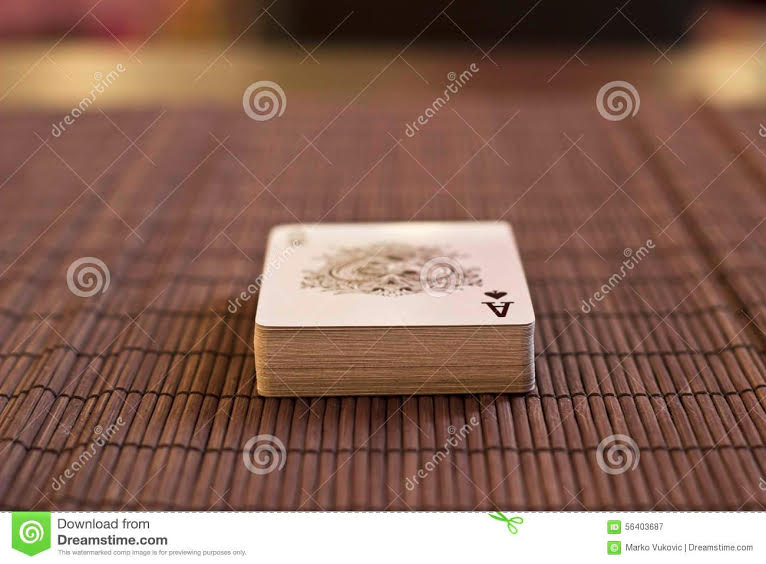
\includegraphics[width=0.2\textwidth]{initialresults/ace_spades_1.jpg}}
  \subfloat[score = 0.73665]{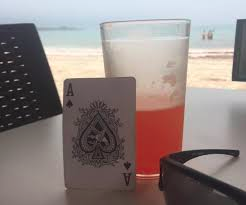
\includegraphics[width=0.2\textwidth]{initialresults/ace_spades_2.png}}

  \subfloat[score = 0.45144]{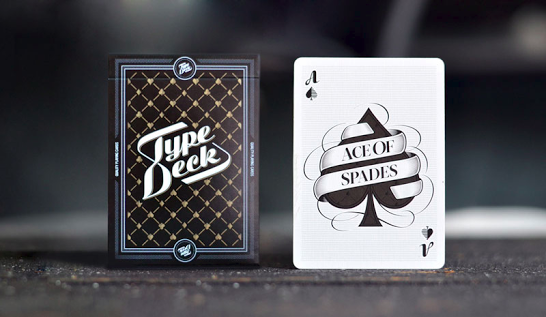
\includegraphics[width=0.2\textwidth]{initialresults/ace_spades_3.png}}
  \subfloat[score = 0.91995]{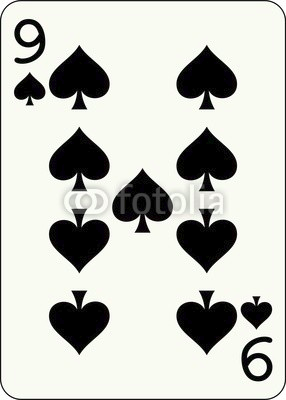
\includegraphics[width=0.2\textwidth]{initialresults/ace_spades_4.png}}
  \caption{\label{fig:initial_results_1} Images correctly classified as having an `Ace of Spades'}
\end{figure}

% card subset =
% 4 of clubs
% 4 of spades
% 4 of hearts
% 4 of spades
% 9 of spades
% A of spades
% A of hearts

One of the things we noticed with this initial test was that the netowrk recognized images with clear backgrounds, but could not recognize cards with complex backgrounds.  Our hypothesis at this point was that the network needed more training data data, and more training steps.

\subsection{Refining the Training}
WIth the success of the initial tests we began to train the network in ernest.  We took the lot of 1800 training images, and ran them through the netowrk using 1600 training steps.  This training took all of a night, but the results were even better.  The network was now able to classify images such as the following.  figure~\ref{fig:refining_results_1} shows some examples of the images with cards that were now correctly classified

\begin{figure}[!tbp]
  \centering
  \subfloat[score = 0.62471]{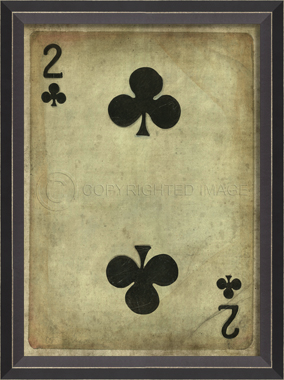
\includegraphics[width=0.2\textwidth]{refining/2_clubs.png}}
  \subfloat[score = 0.79940]{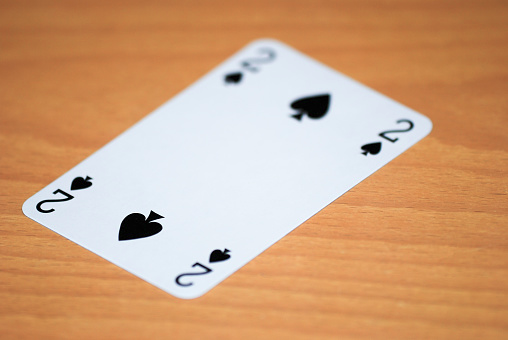
\includegraphics[width=0.2\textwidth]{refining/2_spades.png}}

  \subfloat[score = 0.36798]{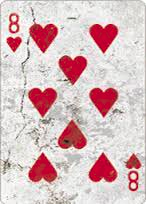
\includegraphics[width=0.2\textwidth]{refining/8_hearts.png}}
  \subfloat[score = 0.69048]{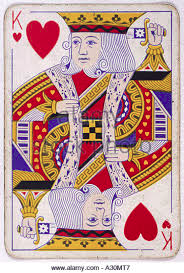
\includegraphics[width=0.2\textwidth]{refining/k_hearts.png}}
  \caption{\label{fig:refining_results_1} Cards with complex backgrounds correctly classified}
\end{figure}



\subsection{OpenCV}
One of our initial goals was to be able to recognize as many situations as we could.  Including cards that were not oriented in a way that our network was trained to handle.  We also wanted to be able to recognize multiple cards within the same image.  What we found was that our network was able to recognize cards oriented horizontally or vertically, it had a hard to with rotated cards, skewed cards, and was terrible with multiplel cards on the same image.  To solve this we thought about training with all orientations of cards, however that would not solve the issue with multiple cards, and would take a long time to create data and train.

Our next solution was to pre process the images.  Try and pull out the cards, and then send those through the trained network.  A library called openCV was used to locate the card within the image, and pull it out.  figure~\ref{fig:opencv_1} shows an example of pre processing and pulling out the playing card portion of the image.

\begin{figure}[!tbp]
  \centering
  \subfloat[OpenCV processing demo]{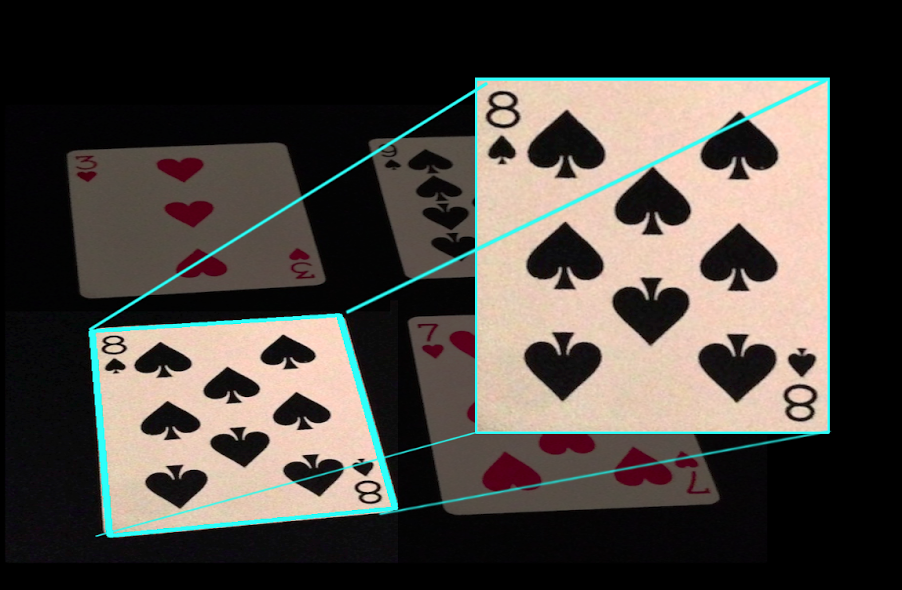
\includegraphics[width=0.4\textwidth]{opencv/demo.png}}

  \subfloat[pre processed ace of spades]{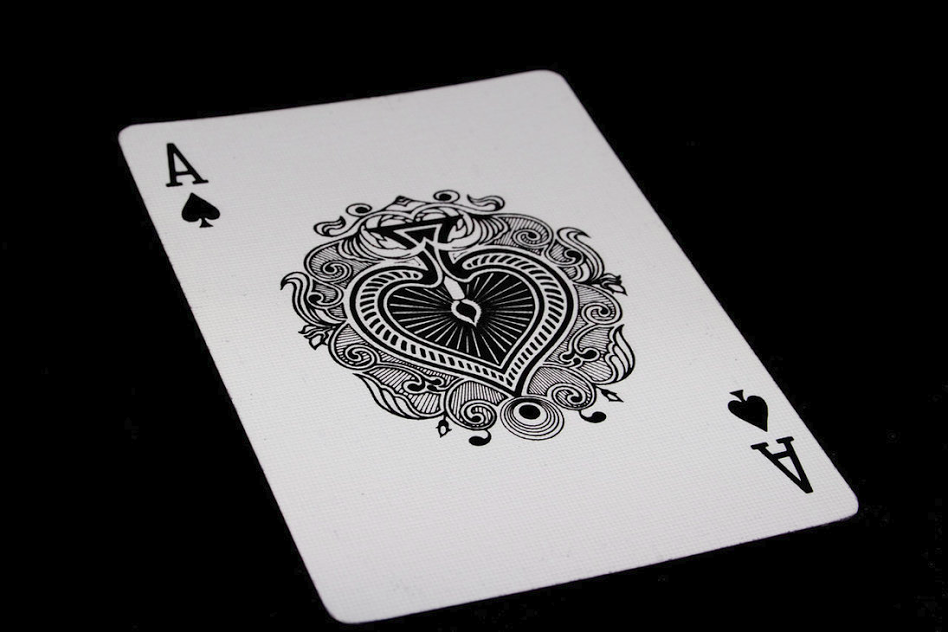
\includegraphics[width=0.2\textwidth]{opencv/ace_spades_1.png}}
  \subfloat[post processed ace of spades]{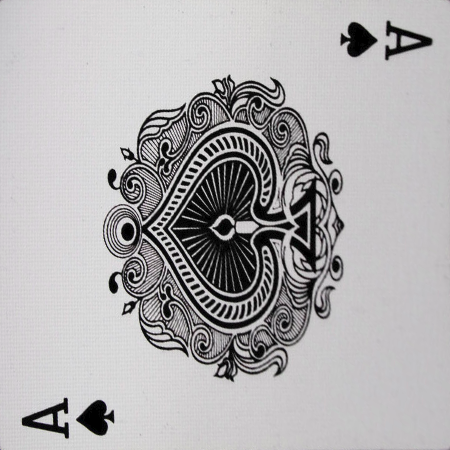
\includegraphics[width=0.2\textwidth]{opencv/ace_spades_2.png}}
  \caption{\label{fig:opencv_1} OpenCV pre processing on images}
\end{figure}


\section{Results and Discussion}

cool graphcs and stuff

\section{Conclusions}

it worked

\nocite{*}
\bibliographystyle{apacite}
\bibliography{references}
\end{document}


